% Created by tikzDevice version 0.7.0 on 2015-04-17 16:39:19
% !TEX encoding = UTF-8 Unicode
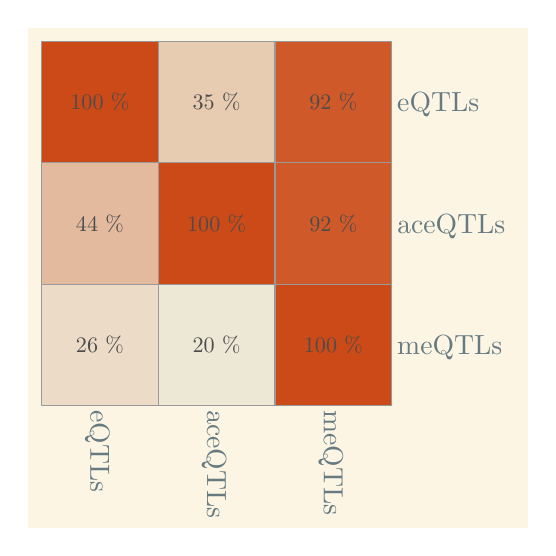
\begin{tikzpicture}[x=1pt,y=1pt]
\definecolor[named]{fillColor}{rgb}{0.99,0.96,0.89}
\path[use as bounding box,fill=fillColor] (0,0) rectangle (180.67,180.67);
\begin{scope}
\path[clip] (  0.00,  0.00) rectangle (180.67,180.67);
\definecolor[named]{drawColor}{rgb}{0.60,0.60,0.60}
\definecolor[named]{fillColor}{rgb}{0.80,0.29,0.09}

\path[draw=drawColor,line width= 0.4pt,line join=round,line cap=round,fill=fillColor] (  5.02,131.80) rectangle ( 47.20,175.66);
\definecolor[named]{fillColor}{rgb}{0.89,0.73,0.62}

\path[draw=drawColor,line width= 0.4pt,line join=round,line cap=round,fill=fillColor] (  5.02, 87.95) rectangle ( 47.20,131.80);
\definecolor[named]{fillColor}{rgb}{0.92,0.86,0.78}

\path[draw=drawColor,line width= 0.4pt,line join=round,line cap=round,fill=fillColor] (  5.02, 44.09) rectangle ( 47.20, 87.95);
\definecolor[named]{drawColor}{rgb}{0.30,0.30,0.30}

\node[text=drawColor,anchor=base,inner sep=0pt, outer sep=0pt, scale=  0.80] at ( 26.11,150.97) {100 \%};

\node[text=drawColor,anchor=base,inner sep=0pt, outer sep=0pt, scale=  0.80] at ( 26.11,107.12) {44 \%};

\node[text=drawColor,anchor=base,inner sep=0pt, outer sep=0pt, scale=  0.80] at ( 26.11, 63.26) {26 \%};
\definecolor[named]{drawColor}{rgb}{0.60,0.60,0.60}
\definecolor[named]{fillColor}{rgb}{0.91,0.80,0.70}

\path[draw=drawColor,line width= 0.4pt,line join=round,line cap=round,fill=fillColor] ( 47.20,131.80) rectangle ( 89.38,175.66);
\definecolor[named]{fillColor}{rgb}{0.80,0.29,0.09}

\path[draw=drawColor,line width= 0.4pt,line join=round,line cap=round,fill=fillColor] ( 47.20, 87.95) rectangle ( 89.38,131.80);
\definecolor[named]{fillColor}{rgb}{0.93,0.91,0.84}

\path[draw=drawColor,line width= 0.4pt,line join=round,line cap=round,fill=fillColor] ( 47.20, 44.09) rectangle ( 89.38, 87.95);
\definecolor[named]{drawColor}{rgb}{0.30,0.30,0.30}

\node[text=drawColor,anchor=base,inner sep=0pt, outer sep=0pt, scale=  0.80] at ( 68.29,150.97) {35 \%};

\node[text=drawColor,anchor=base,inner sep=0pt, outer sep=0pt, scale=  0.80] at ( 68.29,107.12) {100 \%};

\node[text=drawColor,anchor=base,inner sep=0pt, outer sep=0pt, scale=  0.80] at ( 68.29, 63.26) {20 \%};
\definecolor[named]{drawColor}{rgb}{0.60,0.60,0.60}
\definecolor[named]{fillColor}{rgb}{0.81,0.35,0.16}

\path[draw=drawColor,line width= 0.4pt,line join=round,line cap=round,fill=fillColor] ( 89.38,131.80) rectangle (131.56,175.66);

\path[draw=drawColor,line width= 0.4pt,line join=round,line cap=round,fill=fillColor] ( 89.38, 87.95) rectangle (131.56,131.80);
\definecolor[named]{fillColor}{rgb}{0.80,0.29,0.09}

\path[draw=drawColor,line width= 0.4pt,line join=round,line cap=round,fill=fillColor] ( 89.38, 44.09) rectangle (131.56, 87.95);
\definecolor[named]{drawColor}{rgb}{0.30,0.30,0.30}

\node[text=drawColor,anchor=base,inner sep=0pt, outer sep=0pt, scale=  0.80] at (110.47,150.97) {92 \%};

\node[text=drawColor,anchor=base,inner sep=0pt, outer sep=0pt, scale=  0.80] at (110.47,107.12) {92 \%};

\node[text=drawColor,anchor=base,inner sep=0pt, outer sep=0pt, scale=  0.80] at (110.47, 63.26) {100 \%};
\end{scope}
\begin{scope}
\path[clip] (  0.00,  0.00) rectangle (180.67,180.67);
\definecolor[named]{drawColor}{rgb}{0.40,0.48,0.51}

\node[text=drawColor,rotate=270.00,anchor=base west,inner sep=0pt, outer sep=0pt, scale=  1.00] at ( 22.67, 42.33) {eQTLs};

\node[text=drawColor,rotate=270.00,anchor=base west,inner sep=0pt, outer sep=0pt, scale=  1.00] at ( 64.85, 42.33) {aceQTLs};

\node[text=drawColor,rotate=270.00,anchor=base west,inner sep=0pt, outer sep=0pt, scale=  1.00] at (107.03, 42.33) {meQTLs};
\end{scope}
\begin{scope}
\path[clip] (  0.00,  0.00) rectangle (180.67,180.67);
\definecolor[named]{drawColor}{rgb}{0.40,0.48,0.51}

\node[text=drawColor,anchor=base west,inner sep=0pt, outer sep=0pt, scale=  1.00] at (133.53,150.29) {eQTLs};

\node[text=drawColor,anchor=base west,inner sep=0pt, outer sep=0pt, scale=  1.00] at (133.53,106.43) {aceQTLs};

\node[text=drawColor,anchor=base west,inner sep=0pt, outer sep=0pt, scale=  1.00] at (133.53, 62.58) {meQTLs};
\end{scope}
\end{tikzpicture}
